\chapter{二类疾病标记物定位}\label{sec:experiments}
%\section{前言}
在第\ref{sec:method}章中,本文详细介绍了所提出模型的结构、背后的原理、损失函数等内容。接下来,本文将进行相关实验评估。本章将展示本文提出的模型在二类视网膜糖尿病病变数据集和二类模拟皮肤病病变数据集上的相关实验结果。首先在\ref{sec:exper_ds_intro}小节中介绍以上两个用于疾病标记物定位的数据集,包括数据量、类别数量、疾病标记物特点等基本信息。在\ref{sec:exper_evaluation_metrics}小节中,本文将介绍本章实验所选择的实验评价标准(P-R曲线及其AUC)及其原因。\ref{sec:exper_setting}小节将会介绍本章的实验设置,包括学习率、超参数、数据预处理等相关信息。从\ref{sec:bin_dr_ds_experiment}小节开始,本章将展示本文提出的模型在以上两个数据集上的实验结果,包括与CAM和Grad-CAM进行的对比实验和针对本文提出的模型的消融实验。具体来说,在\ref{sec:bin_dr_ds_experiment}小节和\ref{sec:bin_simulated_ds_experiment}小节中,本章将本文提出的方法和CAM以及Grad-CAM进行在两个数据集上的对比实验,通过P-R曲线及其AUC来比较各方法模型的性能表现。在\ref{sec:g_c_g_d_g_d_c_comparsion}小节中,利用二类视网膜糖尿病病变数据集,本章通过分别去掉CNN分类器模块和判别器模块的方式设计消融实验来探究本文提出的模型中的各个子模块所扮演的角色。在\ref{sec:indirect_quantitative_evaluation}小节中,本章基于在理想情况下,将异常图像作为输入,经过编码器-解码器之后的输出图像将极少甚至不再包含疾病标记物,那么这些输出图像将会被分类器分类为正常的设想,通过对比二类视网膜糖尿病病变数据集和经过编码器-解码器的该数据集的分类情况来间接定量评估本文提出的模型的性能表现。\ref{sec:hyper_paras}小节将设置不同的超参数组合,来探究本文提出的模型的鲁棒性。在\ref{sec:dis_arch}小节中,本章将探究不同的判别器网络结构下,本文提出的模型的性能表现,以期读者能对判别器模块更为深刻的认识。接下来,本章将进行以上内容的具体阐述。
\section{数据集介绍}\label{sec:exper_ds_intro}
在本章中,本文将详细介绍本文提出的模型在处理二类问题时的性能表现。在\ref{sec:usually_ds_intro}小节中,本文介绍了包括眼底病变数据集和黑色素瘤皮肤病病变数据集在内的诸多可用于疾病标记物定位任务的常见数据集。考虑到本文的研究内容是疾病标记物分布比较分散、疾病标记物尺寸大小不一的疾病标记物定位任务(黑色素瘤皮肤病病变图像中的异常区域所占比例通常在$1/3$以上且往往没有专门的正常图像),本文将使用包括二类视网膜糖尿病病变数据集(\ref{subsec:bin_dr_ds}小节)和二类模拟皮肤病病变数据集(\ref{subsec:bin_simulated_skin_ds}小节)在内的两个数据集来评估我们提出的模型用于疾病标记物定位的表现。因此,在实验评估之前非常有必要先详细介绍以上两个数据集,以便让读者对于本文要解决的问题能有更为清晰的认识与更为明了的理解。下面将进行相关内容的具体叙述。
\subsection{二类视网膜糖尿病病变数据集}\label{subsec:bin_dr_ds}
二类视网膜糖尿病病变数据集是来自Kaggle视网膜糖尿病病变数据集(相关描述请参见\ref{subsec:original_dr_dataset_intro}小节),该数据集由从原始Kaggle视网膜糖尿病病变数据集中随机选择出来的$2,101$张异常图像和$2,101$张正常图像组成,尺寸大小为$128\times 128$。部分图像示例如图\ref{subfig:bin_dr_ds_example}所示。每张图像中明显比周围要亮的圆形区域为视盘,为共有结构,而有些图像视盘在左边,有些视盘在右边,这是因为有些图像是左眼眼底图像,而有些是右眼眼底图像。眼底图像还含有丰富的血管,呈现一种随机走向,并且包含非常丰富的毛细血管网,另外,图像之间的背景亮度有较大差别,比如,图中第一行第三列图像背景较亮,而第二列第一行图像背景较暗。就疾病标记物本身来说,也呈现一种分散、大小不一、不够明显而又难以被察觉的特点,而且还能发现,疾病标记物本身的颜色与背景颜色比较相近,比如图中的第二列第三行和第一列第三行图像,因此这些疾病标记物很容易与背景相混淆,这些特点都表明在该数据集上完成疾病标记物定位的任务极具挑战性。由于在该数据集上进行像素级标注代价高昂,我们选择随机选出$40$张眼底图像并邀请两位专业眼科医师对其进行像素级标注,用于后续章节中对实验的定量分析,以增加实验结果的有效性与可信度。

%另外,为了在后续章节中说明本文模型方法的有效性以及增加实验结果的可信度;但是,Kaggle视网膜糖尿病病变数据集本身没有像素级标注而在所有的异常图像中标出所有疾病标记物的精确位置又是极其昂贵的,我们选取了这种方案,随机选出了40张眼底图像并请两位专业眼科医师对其中所有的疾病标记物进行了像素级标注,用于后续章节的定量分析。


%从图\ref{subfig:bin_dr_ds_example}可以看出,眼底图像中含有丰富的血管,呈现一种随机走向,并且包含非常丰富的毛细血管网,这种充分而又精细的血管纹理细节本身就给图像的重建增加了困难,而图像重建只是本文模型方法中最为基础的一步。我们注意到视网膜糖尿病性病变图像中的血管所在像素位置的梯度明显高于周围像素,为了让编码器-解码器重建图像更为容易,本文使用Sobel梯度算子~\cite{sobel2014history}沿着水平和竖直两个方向的提取图像每个像素的梯度,将其作为L1损失函数的权重。另外,图像之间的背景亮度有较大差别,比如,图\ref{subfig:bin_dr_ds_example}中,第一行第三列图像背景较亮,而第二列第一行图像背景较暗。就疾病标记物本身来说,也呈现一种分散、大小不一、不够明显而又难以被察觉的特点,而且还能发现,疾病标记物本身的颜色与背景颜色比较相近,比如图\ref{subfig:bin_dr_ds_example}中的第二列第三行和第一列第三行图像,因此这些疾病标记物很容易与背景相混淆,这也是在二类视网膜糖尿病病变数据集上完成疾病标记物精确定位任务最大的难点。二类视网膜糖尿病性病变图像的这些特点都表明在该数据集上完成疾病标记物定位的任务极具挑战性。另外,视网膜糖尿病性病变也是当今导致病人失明的主要原因,说明了该任务的具有较大现实意义和应用潜能。注意,有些疾病标记物的边界不仅呈现一种不规则状况,边界还十分模糊,用矩形框圈出疾病标记物的位置相对比较容易,但是做出像素级精确标注却比较难,这也是本文只随机选出40张图像做像素级标注的主要原因。

\subsection{二类模拟皮肤病病变数据集}\label{subsec:bin_simulated_skin_ds}
二类模拟皮肤病病变数据集包含带有人工疾病标记物的皮肤图像。为了生成这个数据集,我们首先从一个皮肤镜图像数据集~\cite{codella2018skin}(原始数据集相关内容介绍可参见\ref{subsec:original_dermatoscope_ds_intro}小节)中提取了$2,920$张图像尺寸大小为$128\times128$的正常图像(实际上是通过滑动窗口方式得到的图像区域块)。为了模拟真实皮肤图像中生物标志物的数量、大小和所在位置的随机变化,我们通过随机参数控制,在每个模拟皮肤图像的一定范围内随机生成这些参数的值。更具体地说,对于每张异常图像,从Image-Net数据集~\cite{deng2009imagenet}中随机选择一到三张图像,并将其调整为尺寸大小为$4\times 4$、$8\times 8$或$16\times 16$的缩略图。再将缩略图嵌入到皮肤图像中,最后将其局部平滑作为人工生物标记。最终,二类模拟皮肤病病变数据集中共有异常图像$1,310$张,正常图像$1,460$张。注意,此数据集中的所有异常图像的人工疾病标记物都有像素级的标注。

从图\ref{subfig:bin_simulate_skin_example}中可以看出,二类模拟皮肤病病变数据集中背景差异比较大,主要表现在颜色和亮度,比如图中第二行第三列图像背景为红色,较亮,而第一行第二列图像背景则较暗。注意,由于本文对于所有异常图像中的疾病标记物都做了局部平滑处理,故此数据集中的疾病标记物也显得比较真实,最为明显的特点是其边界比较模糊。再加上引入了疾病标记物大小、数量和位置这三个随机变化量,这也大大增加了在此数据集上实现疾病标记物的精确定位的难度。与二类视网膜糖尿病病变数据集相比,虽然疾病标记物在纹理结构上并没有前者复杂,但是二类模拟皮肤病病变数据集的优势在于拥有所有疾病标记物的像素级标注,故可在整个数据集上进行全面的定性分析,来反应出各个模型方法在疾病标记物精确定位任务上的性能表现,而二类模拟皮肤病病变数据集本身的模拟疾病标记物也比较接近真实,从而保证了从该数据集得出的实验结果的可行性和可靠性,这也是设置该数据集的意义所在。
\begin{figure}[h]
	\centering
	\begin{subfigure}{0.48\textwidth}
		\centering
		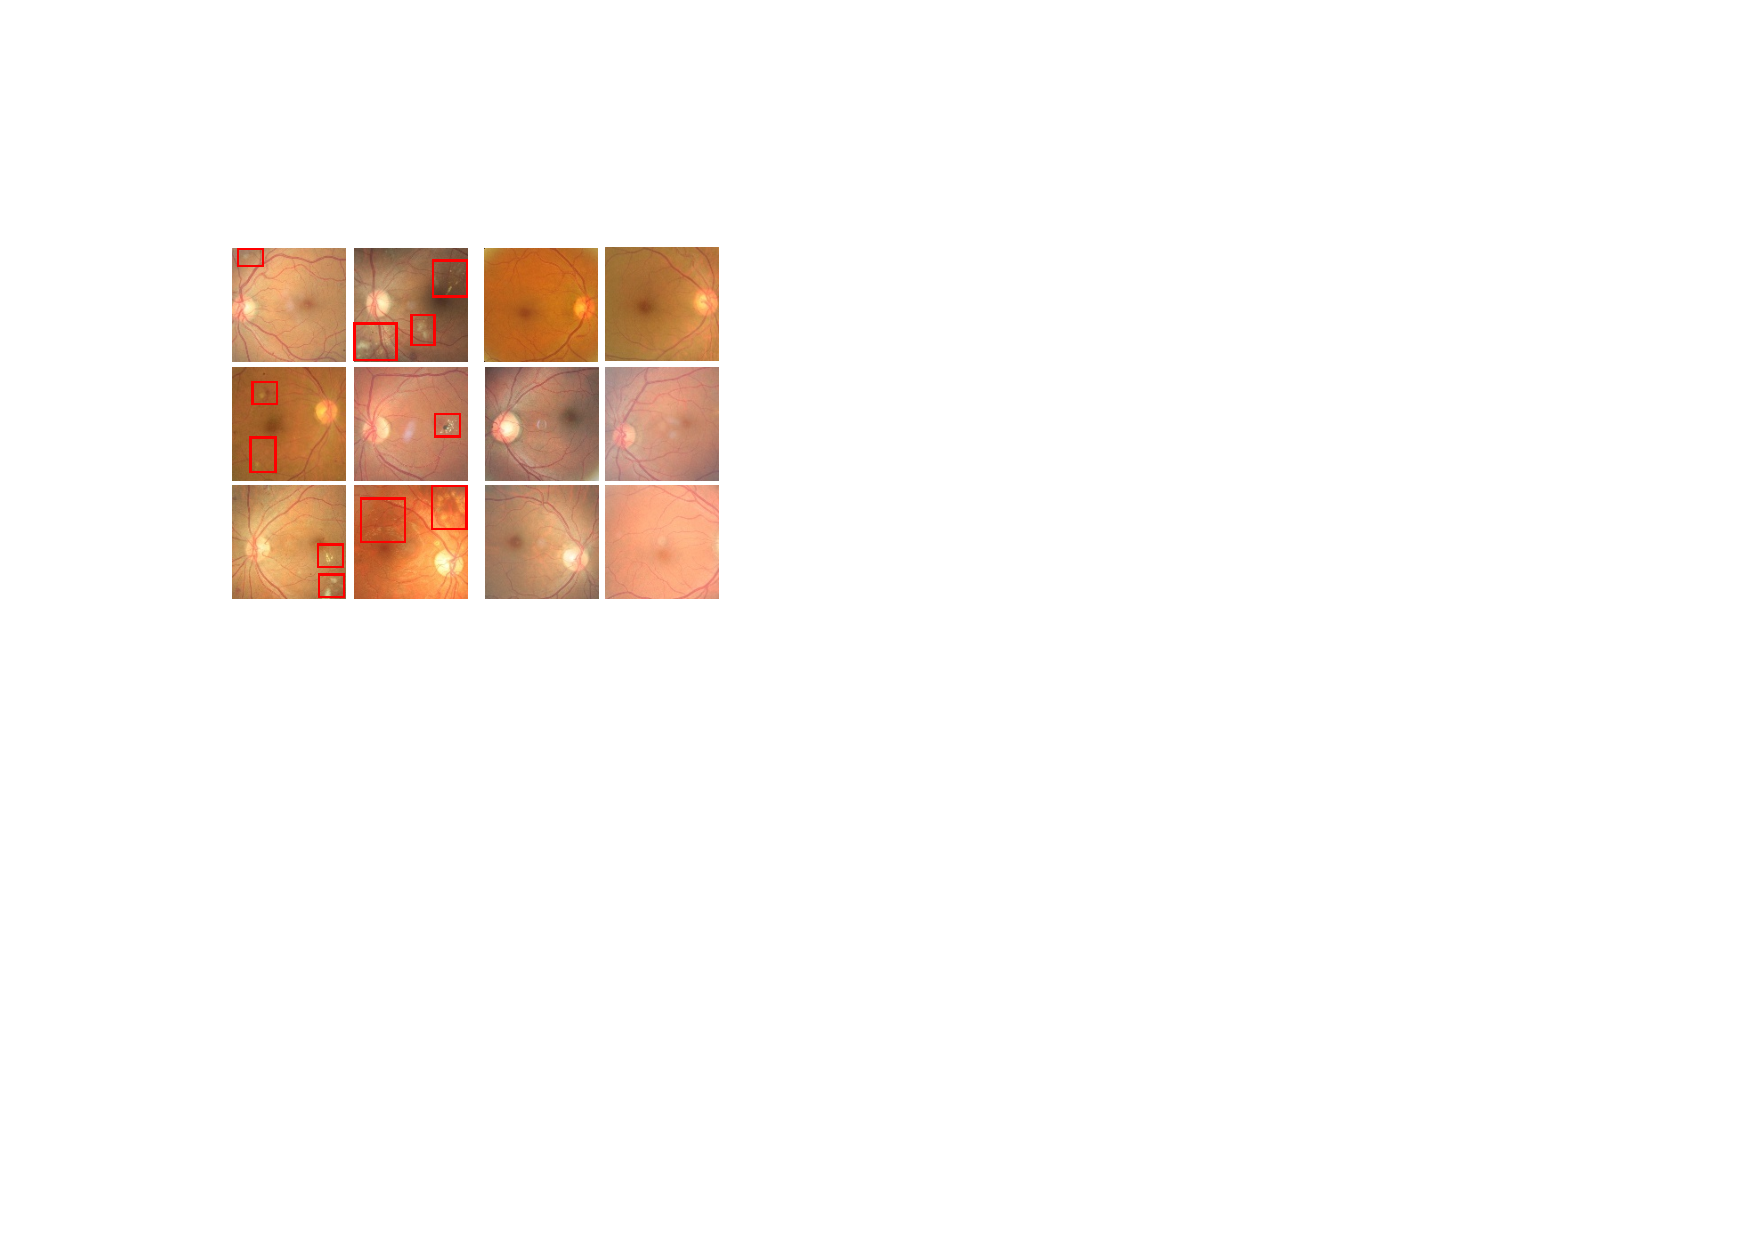
\includegraphics[width=1\textwidth]{figure/bin_dr_ds_example}
		\caption{二类视网膜糖尿病病变数据集部分图像示例(第1、2列是异常图像,第3、4列是正常图像)}
		\label{subfig:bin_dr_ds_example}
	\end{subfigure}
	\quad
	\begin{subfigure}{0.48\textwidth}
		\centering
		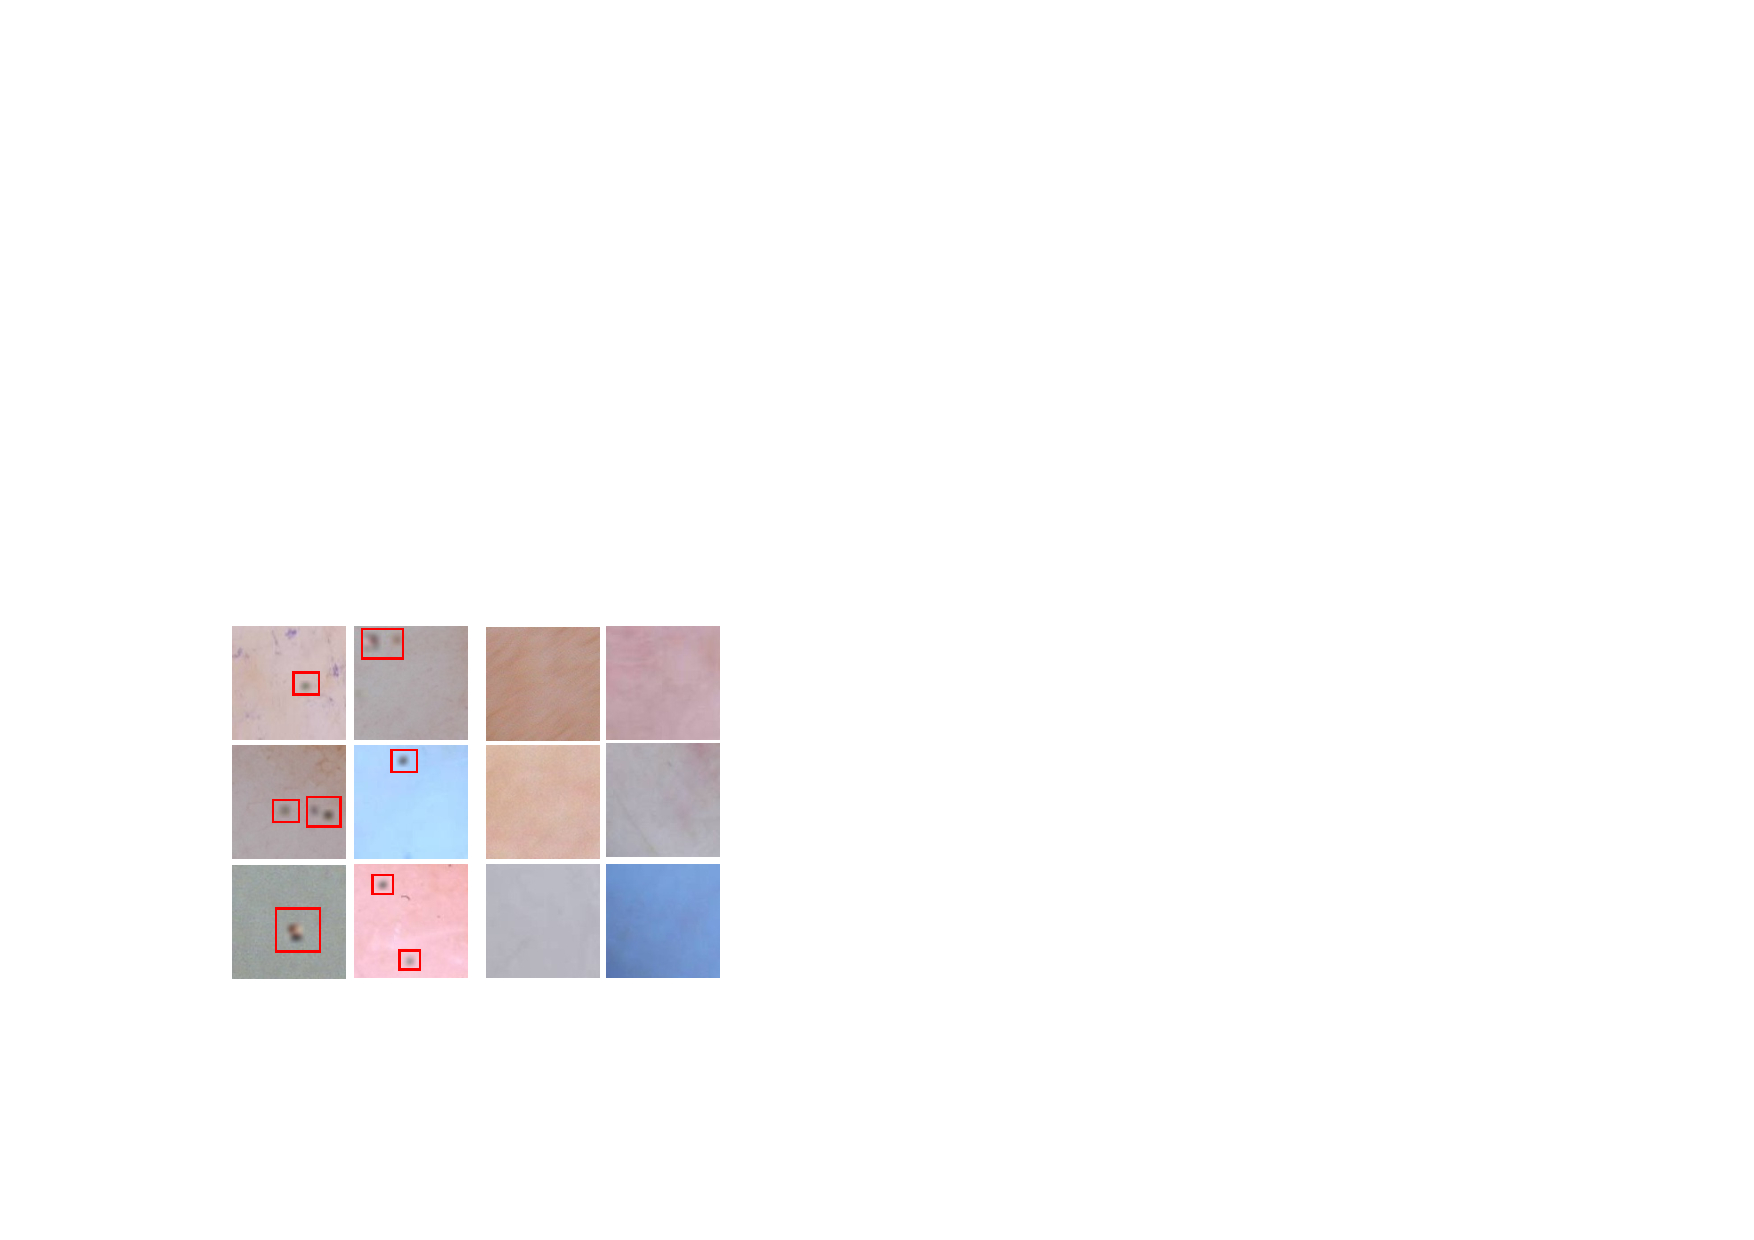
\includegraphics[width=1\textwidth]{figure/bin_simulate_skin_example}
		\caption{二类模拟皮肤病病变数据集部分图像示例(第1、2列是异常图像,第3、4列是正常图像)}
		\label{subfig:bin_simulate_skin_example}
	\end{subfigure}
	\caption{本文实验数据集部分图像示例(红色矩形框表示疾病标记物)}
	\label{mul_fig:bin_ds_example}
\end{figure}
\section{评价标准}\label{sec:exper_evaluation_metrics}

%在\ref{subsec:roc_curve}小节和\ref{subsec:pr_curve}小节中,本文分别介绍了ROC曲线及其AUC和P-R曲线及其AUC,并在此过程中定义了FPR、TPR等相关概念。本文还在\ref{subsec:pr_curve}小节中说明了ROC曲线对正负样本分布的变化表现比较稳定,而P-R曲线在此情况下则更为敏感,故P-R曲线更能反映出在正负样本比例悬殊较大情况下系统的真实性能。
在\ref{sec:evaluation_metrics}小节中,本文分别介绍了ROC曲线和P-R曲线及其各自AUC,并说明了在正负样本比例悬殊较大情况下,P-R曲线更能反映出系统的真实分类性能。从表\ref{tab:bin_ds_pixel_freqs}可以看出,无论是二类视网膜糖尿病病变数据集还是二类模拟皮肤病病变数据集,异常像素(正样本)和正常像素数量(负样本)之间的比例存在巨大悬殊甚至达到$88:1$(二类视网膜糖尿病病变数据集),故接下来的实验均采用P-R曲线及其AUC作为主要评价标准,但是ROC曲线也会在本文附录\ref{chapter:append1}中进行展示,实验评估从而更为全面,对相关内容感兴趣的读者可自行查看。

对于正常图像输入,我们期望编码器-解码器输出仍保持正常,反之,对于异常图像输入,我们期望编码器-解码器能将其转化为正常图像输出。为此,本文引入特异性(Specificity)和召回率(Recall)分别来衡量经过编码器-解码器之后的正常图像的保持率和经过编码器-解码器的异常图像的转化率。

\begin{table}[h]
	\centering
	%\caption{二类视网膜糖尿病病变数据集和二类模拟皮肤病病变数据集正负像素数量统计表}
	\caption{两个实验数据集正负像素数量统计表}
	\label{tab:bin_ds_pixel_freqs}
	\begin{tabular}{c|c|c|c}
		\toprule[2pt]
		数据集名称 & 正常像素数量 & 异常像素数量 & 比例 \\
		\midrule[2pt]
		二类视网膜糖尿病病变数据集&  $643,837$ & $11,523$ & $\simeq 56: 1$ \\ \hline
		二类模拟皮肤病病变数据集 & $21,222,487$ & $240,553$ & $\simeq 88: 1$ \\
		\bottomrule[2pt]
	\end{tabular}
\end{table}


\section{实验设置}\label{sec:exper_setting}

本文所有实验相关代码实现均采用当前流行的深度学习框架PyTorch\footnote{https://pytorch.org/}。编码器-解码器模块选择一个经过修改的U-Net~\cite{iglovikov2018ternausnet}(详细结构修改请参见\ref{subsec:encoder_decoder_model}小节)。CNN分类模块采用Resnet-18,判别器模块使用一个$7$层卷积神经网络($4$个DownConv2d模块+$3$个Conv2dBlock模块,更直观地模型结构请对照图\ref{fig:discrimintor_architecture})。GAN采用WGAN-GP。为了让U-Net更好地重构图像,本文先将U-Net在数据集上进行预训练。

在预处理阶段,对于二类视网膜糖尿病病变数据集,我们先将图像中没有信息的四个黑角去掉;另外,由于眼底图像中的视网膜基本是呈圆形的,我们提取了视网膜的边界再根据视网膜边界取其最大内接矩形,从而彻底去掉眼底图像中的不包含任何信息的黑色部分,最后将图像尺寸大小重新调整到$128\times128$,最终得到二类视网膜糖尿病病变数据集。在图像数据送入模型训练之前,我们将输入减去$0.5$随后除以$0.5$,将输入变换到$[-1,1]$。在实验超参数设定方面,WGAN-GP中的梯度惩罚系数$\lambda$被设置为$10$(与WGAN-GP原文中一致)。模型训练使用Adam优化器~\cite{kingma2014adam},其中,对于CNN分类器,$\beta1$和$\beta2$分别设为$0.9$和$0.999$,对于生成器和判别器,$\beta1$和$\beta_2$分别设为$0.3$和$0.9$,默认学习率取$0.0002$,训练每次迭代取32张图像。对于所有的测试,$\lambda_1 = 0.4$和$\lambda_{2} = 10.0$。在生成P-R曲线之前,定位结果的热图被归一化为$[0,1]$。

%请注意,ROC曲线并不适合用来评价疾病标记物的定位性能,因为每个数据集的正、负像素的比例非常不平衡(参考表$\ref{tab:bin_ds_pixel_freqs}$)。因此,本文正文中只展示相关实验的P-R曲线。

请注意,我们的目标是通过图像级标签从已有图像中搜索和定位生物生物标记(像素级),而不是训练模型从新图像中寻找疾病标记物。因此,对于每个数据集,所有的图像都被用来训练我们的模型,然后对模型进行定性和定量的评估。因此,我们没有设置额外的验证集,将在相同的数据集上训练和评估我们的模型。基于同样的原因,在训练阶段,我们也没有采用随机翻转、随机裁剪等数据增广手段。

\section{在二类视网膜糖尿病病变数据集上的疾病标记物定位}\label{sec:bin_dr_ds_experiment}
本节将展示本文提出的模型在视网膜糖尿病病变数据集上的实验结果,本文提出的模型将与CAM和Grad-CAM共计两种用于卷积神经网络可视化方法作定性分析和定量分析。

CAM和Grad-CAM最为一种用于CNN可视化的方法,本身需要分两步完成。需要先训练得到一个分类器,再通过特征图的可视化来间接完成疾病标记物的定位。一方面为了尽量减少与实验内容无关的因素干扰,另一方面由于CAM只能完成对最后一层是全局均值池化层的卷积神经网络的可视化(相关解释可参见\ref{subsec:gradient_based_methods}小节),综合以上因素,本文将ResNet-18作为CAM和Grad-CAM可视化的目标CNN分类器。另外,为了排除由于CNN性能的缺陷导致可视化结果表现较差,本文同样使用数据集中的所有图像来训练ResNet-18分类器,即没有为ResNet-18单独设置测试集,本文后续所有关于CAM和Grad-CAM的相关实验结果均在此条件设置下完成。在使用视网膜糖尿病病变数据集训练ResNet-18时,分类器最终的分类准确率达到了100\%。由于Grad-CAM可对任意层输出的特征图完成可视化,从而实现疾病标记物的定位。如图\ref{fig:retinal_image_res}所示,本文展示出了使用Grad-CAM对中间层特征输出(第$4$列)和最后一层特征输出(第$5$列)的疾病标记物定位结果(可与CAM作比较)。
\begin{figure}[h]
	\centering
	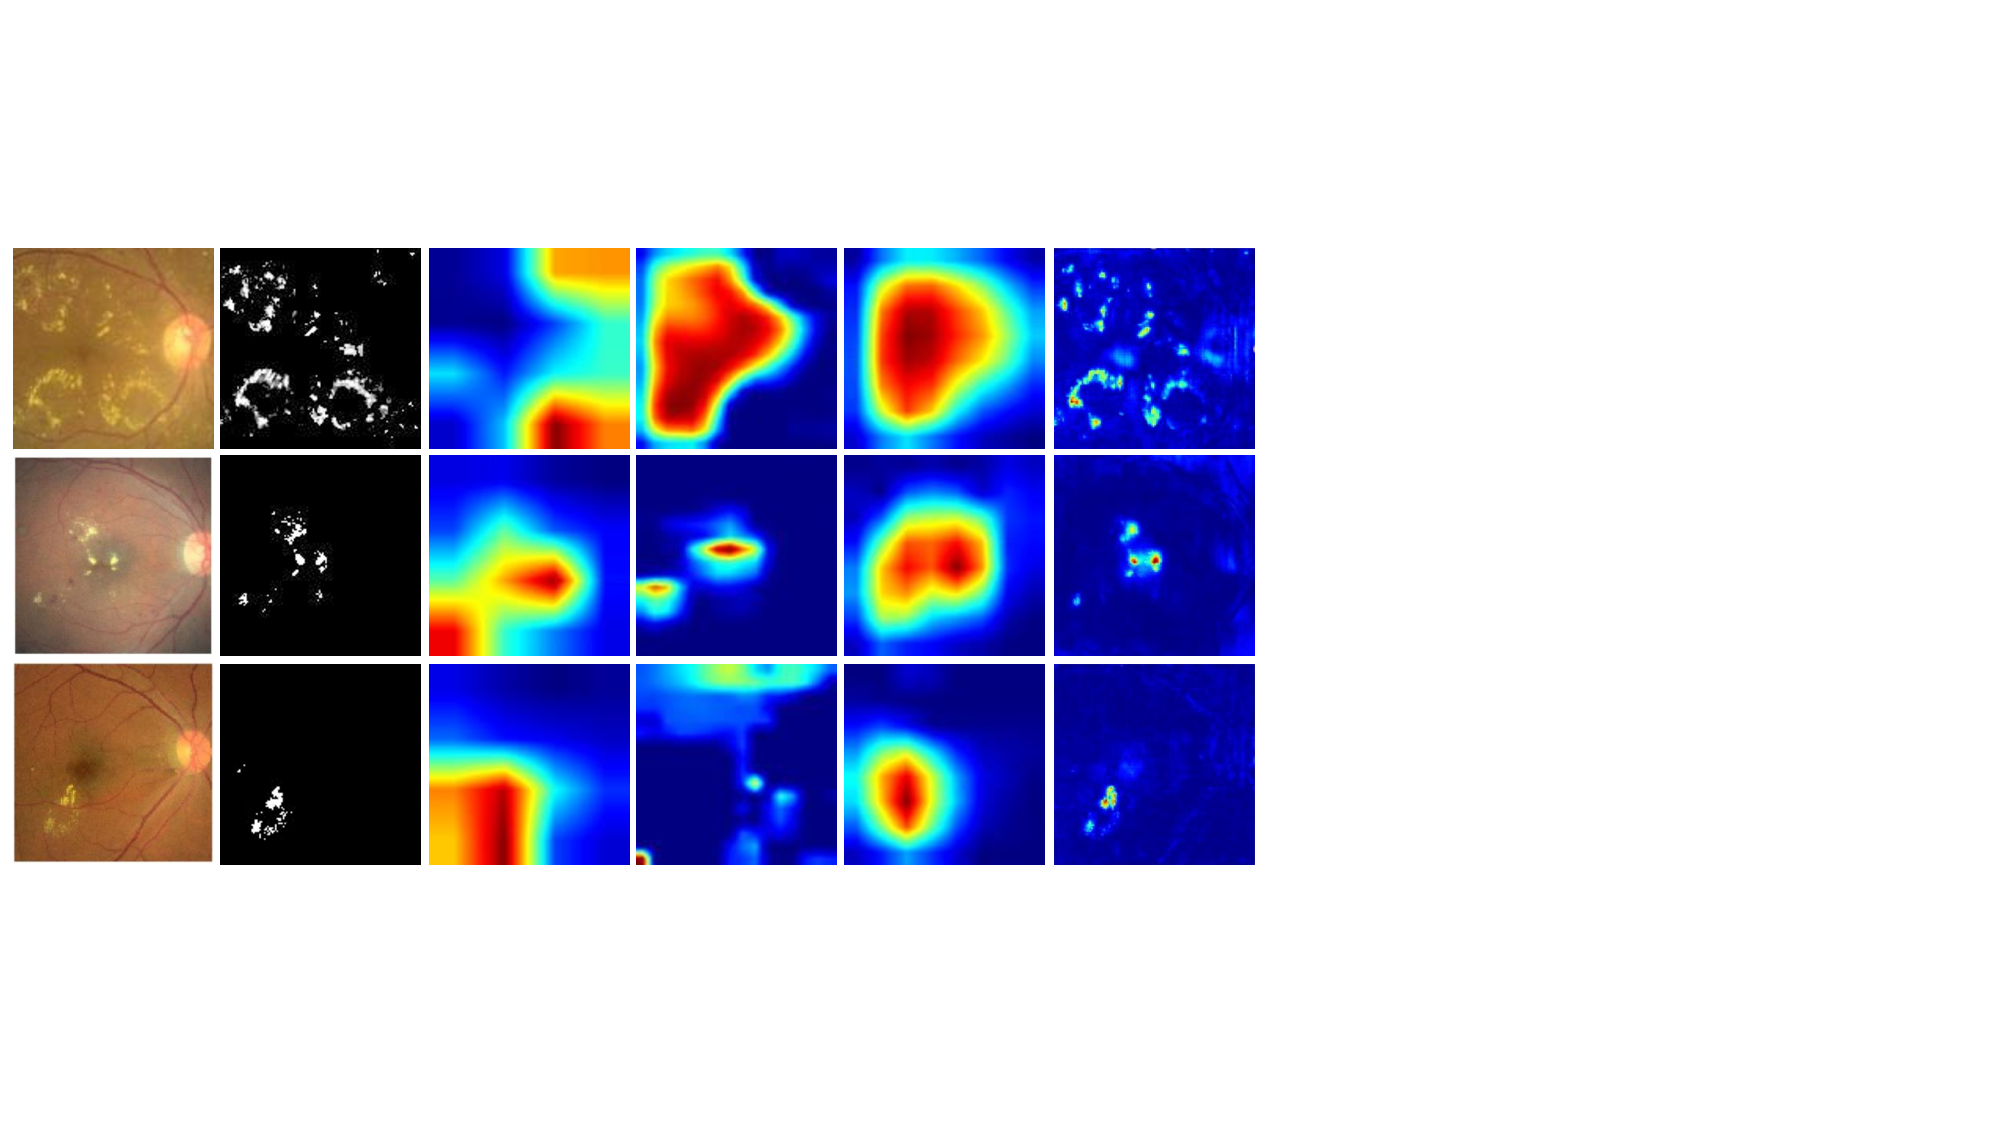
\includegraphics[width=1.0\textwidth]{figure/retinal_image_res.pdf}
	\caption{在二类视网膜糖尿病病变数据集上疾病标记物定位热图对比}
	\label{fig:retinal_image_res}
\end{figure}

如图\ref{fig:retinal_image_res}所示,图中第$1$列表示原始异常图像,第$2$列表示其像素级标注,第$3$列表示CAM的定位结果,第$4$列表示Grad-CAM使用分类器中间层的特征图可视化的定位结果(Grad-CAM-1),第$5$列表示Grad-CAM使用分类器最后一层特征图可视化的定位结果(Grad-CAM-2),第$6$列是本文提出模型的定位结果。第$3-6$列表示输入图像的定位结果的热图,图中某一区域颜色越红,表示该区域为疾病标记物的可能性越高。蓝色表示的意义与红色相反,表示其所在区域是疾病标记物的可能性越低。以上颜色代表的意义同样适用于下文所有热图。

从图中第$3$列定位结果可以看出,虽然CAM发现的疾病标记物或者说异常区域最多,但是CAM也将周边区域作为疾病标记物的一部分。这主要是由于将最后一个卷积层($4\times 4$)的输出向上采样到图像大小($128\times 128$)。另外,CAM也未能检测到第一幅图像(第$3$列,第$1$行)中的大部分异常区域。Grad-CAM作为CAM的扩展,它允许我们从多个层生成可视化的解释,例如中间卷积层(第$4$列,可记为Grad-CAM-1)和最后卷积层(第$5$列,可记为Grad-CAM-2)。虽然Grad-CAM-1在第$4$列(第三幅图像)获得了较为准确的疾病标记物定位结果,但通过也将正常区域(图像中中间上方区域和左下角区域)误认作包含疾病标记物的异常区域。更多的是其结果要么不够精确(第$1$行),要么不够精确(第$2$行和第$3$行)。与CAM相比,Grad-CAM-1实现了更为精确的定位结果,证明了其优于CAM的性能。另外,同样是由于对可视化特征图悬殊的上采样倍数($4\times 4 \rightarrow 128\times 128$),可以发现,Grad-CAM-2(第$5$列)标记的区域和CAM(第$3$列)没有太大区别。相比之下,本文提出的方法对形状不规则、分布分散的疾病标记物进行了更精确的局部化(第$6$列),从定性分析的角度证明了其优于CAM和Grad-CAM的性能。
\begin{figure}[h!]
	\centering
	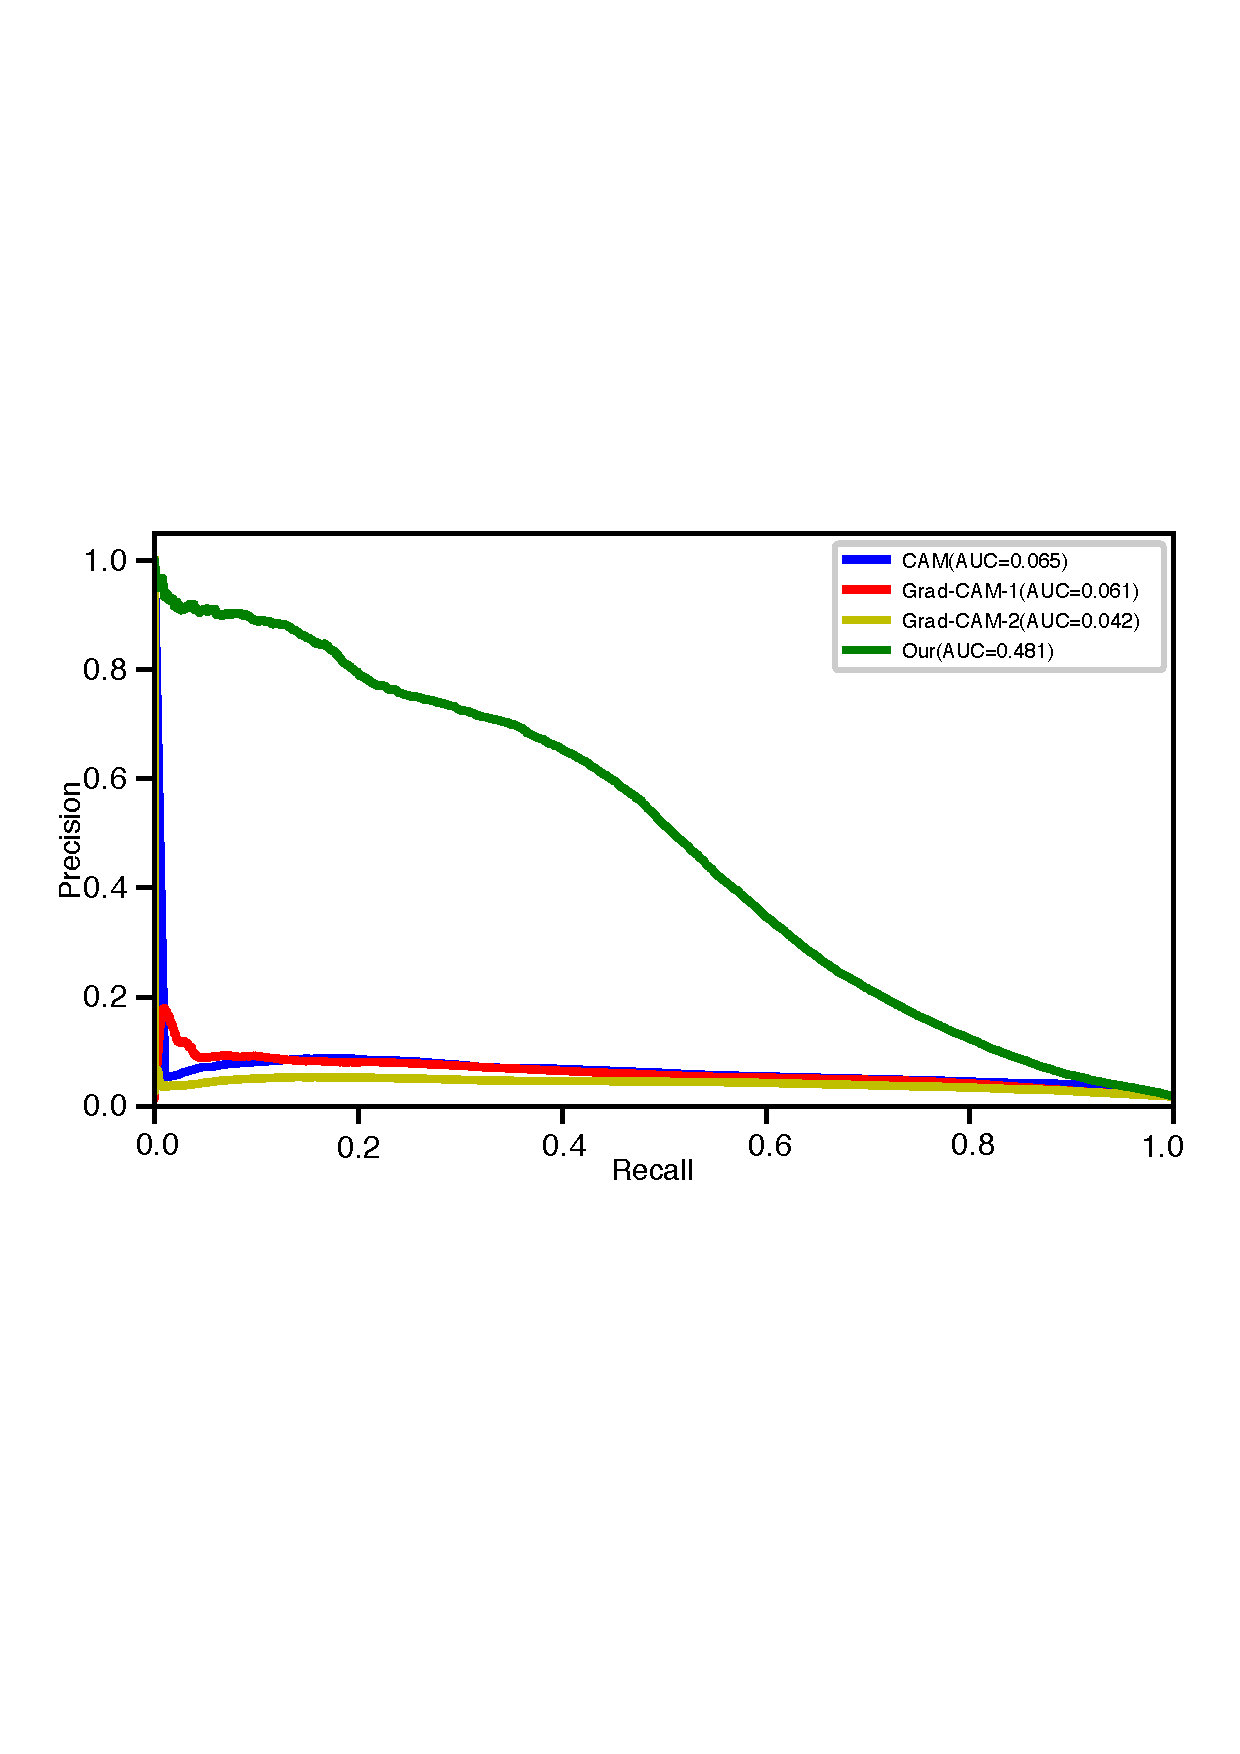
\includegraphics[width=1.0\textwidth]{figure/pr_curve_retinal_image/pr_curve}
	\caption{在$40$张视网膜糖尿病病变图像上P-R曲线对比}
	\label{fig:retinal_image_pr_curve}
\end{figure}

另外,本文充分利用二类视网膜糖尿病病变数据集中的$40$张像素级标注,通过对每种方法的定量评价,本文提出的模型、CAM、Grad-CAM-1和Grad-CAM-2的P-R曲线如图\ref{fig:retinal_image_pr_curve}所示。可以发现,绿色P-R曲线在其他三条曲线的上方,且与下侧横轴和左侧纵轴围成的封闭区域面积显然最大。以上四种方法各自对应的P-R曲线下的面积(AUC)分别为$0.481$,$0.065$,$0.061$和$0.042$,从而进一步从定量分析的角度证明了本文提出的模型在二类视网膜糖尿病病变数据集上的性能优越性。

\section{在二类模拟皮肤病病变数据集上的疾病标记物定位}\label{sec:bin_simulated_ds_experiment}
本节将展示本文提出的模型在模拟皮肤病病变数据集上的实验结果分析,本文提出的模型的比较对象同样是与CAM和Grad-CAM共计两种CNN可视化方法进行比较,分定量分析和定性分析两个角度展开。

与\ref{sec:bin_dr_ds_experiment}小节一样,在本实验中,依然将ResNet-18作为CAM和Grad-CAM可视化的目标CNN分类器,同样没有单独设置测试集,分类器最终CNN分类准确率均达到了$99.7\%$以上。类似的,由于Grad-CAM可对卷积神经网络的任意层输出特征进行可视化,故在此实验中,同样选择了中间层输出特征和最后一层输出特征进行可视化。
\begin{figure}[h]
	\centering
	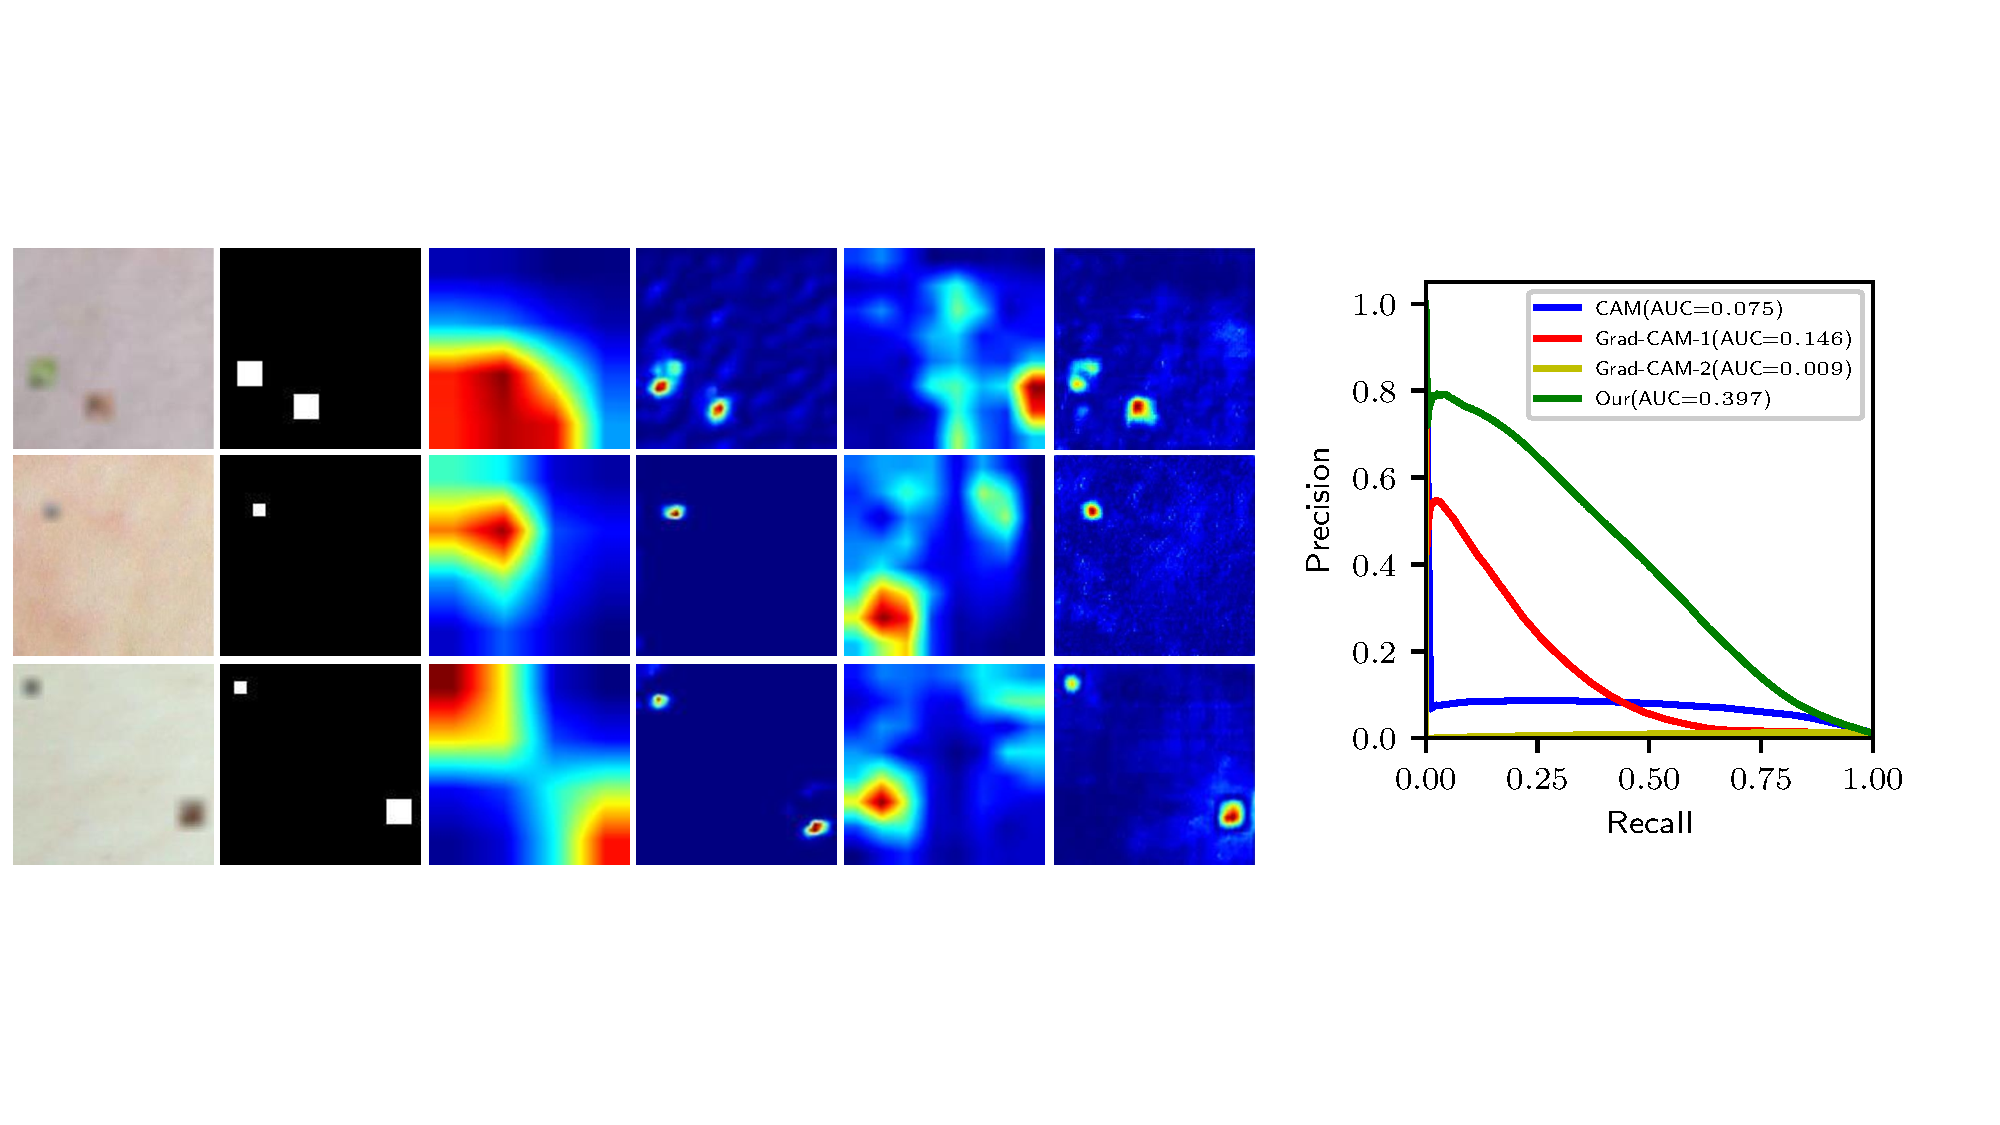
\includegraphics[width=1.0\textwidth]{figure/pr_curve_skin_image.pdf}
	\caption{在二类模拟皮肤病病变数据集上疾病标记物定位热图对比} 
	\label{fig:simulated_skin}
\end{figure}

如图\ref{fig:simulated_skin}所示,图中第$1$列表示原始异常图像,第$2$列表示其像素级标注,第$3$列表示CAM的定位结果,第$4$列表示Grad-CAM使用分类器中间层的特征图可视化的定位结果(Grad-CAM-1),第$5$列表示Grad-CAM使用分类器最后一层特征图可视化的定位结果(Grad-CAM-2),第$6$列是本文提出模型的定位结果。

从图\ref{fig:simulated_skin}可以看出,人工模拟生物标志物的皮肤图像进一步证实了本文提出的模型的优越性能。从图\ref{fig:simulated_skin}第$6$列可以看出,本文提出的方法几乎可以完美、精确地定位人工疾病标记物,而CAM(第$3$列)和Grad-CAM(第$4$列和第$5$列)的性能再次表现出劣势。从总体上来说,第$4$列中疾病标记物定位结果明显要比第$3$列更精确、更完美,也就能说明Grad-CAM在定位疾病标记物上优于CAM。同样是由于特征图的过度上采样,CAM(第$3$列)和Grad-CAM-2(第$5$列)呈现类似的定位结果:虽然能检测到疾病标记物的位置,但同时也包含了疾病标记物周围的大量正常像素。之所以Grad-CAM-1(第$4$列)基本能精确定位到疾病标记物的位置而极少包含疾病标记物的周围像素,主要是因为Grad-CAM-1是通过对ResNet-18中第一个卷积层的特征输出的可视化结果来完成疾病标记物的定位,其中上采样倍数较小($64\times 64\rightarrow 128\times 128$),这也能从侧面说明在该数据集上定位疾病标记物要比在二类视网膜糖尿病病变数据集上容易得多(浅层特征便具备高级语义)。而CAM和Grad-CAM-2却都选择了最后一层卷积层的输出特征,其中上采样倍数要大得多($4\times4\rightarrow 128\times 128$)。
\begin{figure}[h]
	\centering
	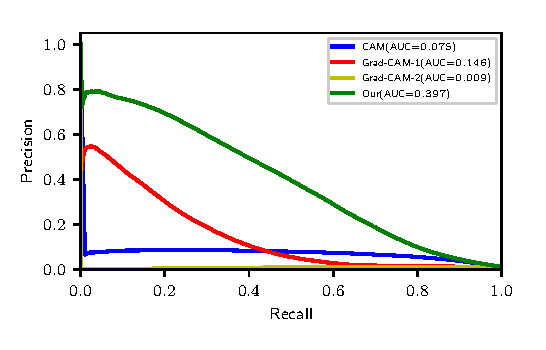
\includegraphics[width=1.0\textwidth]{figure/pr_curve_skin_image/pr_curve}
	\caption{在二类模拟皮肤病病变数据集上P-R曲线对比}
	\label{fig:simulated_skin_pr_curve}
\end{figure}

与CAM和Grad-CAM相比,图\ref{fig:simulated_skin}从定性分析的角度证明了本文提出的方法在二类模拟皮肤病病变数据集上的性能优越性,图\ref{fig:simulated_skin_pr_curve}再次从定性分析的角度证明了这一结论。CAM、Grad-CAM-1、Grad-CAM-2和本文提出的模型根据二类模拟皮肤病病变数据集上所有标注所得出的P-R曲线如图\ref{fig:simulated_skin_pr_curve}所示。不难看出,图中绿色曲线明显在其他三条曲线的上方,与下侧横轴和左侧纵轴围成的封闭区域的面积上,绿色曲线也明显大于其他三条曲线。以上四种方法各自对应的P-R曲线的AUC分别是$0.075$、$0.146$、$0.009$和$0.397$。
\section{CNN分类器和判别器角色探究}\label{sec:g_c_g_d_g_d_c_comparsion}
在\ref{sec:bin_dr_ds_experiment}小节和\ref{sec:bin_simulated_ds_experiment}小节中,本文通过定性分析和定量分析两个角度在二类视网膜糖尿病病变数据集和二类模拟皮肤病病变数据集上证明了本文提出的模型在疾病标记物定位上的优越性能。为了进一步探究本文提出的模型中各个子模块在视网膜糖尿病病变图中扮演的角色以及添加的必要性(相关内容参见\ref{subsec:model_architecture}小节),本节内容将完成消融实验,分别去掉本文提出的模型中的CNN分类器和判别器,以探究CNN分类器模块和判别器模块的在整个模型中所起的作用。为了方便后续内容叙述,对于本文提出的模型,本文将其记为G-D-C模型,将移除判别器模块之后的模型记作编码器-解码器-CNN分类器(G-C)模型,将移除CNN分类器模块之后的模型记作编码器-解码器-判别器G-D模型。G-D-C模型、G-C模型和G-D模型的在二类视网膜糖尿病病变数据集上的部分实验结果如图\ref{fig:u_d_c_comparation}所示。
\begin{figure}[h]
	\centering
	\includegraphics[width=1.0\textwidth]{figure/u_d_c_comparation.pdf}
	\caption{G-D-C模型、G-C模型和G-D模型定位热图对比} 
	\label{fig:u_d_c_comparation}
\end{figure}

如图\ref{fig:u_d_c_comparation}所示,第$1$列是原始输入图像,其中第一行是正常图像输入,第$2-4$行是异常图像输入。第$2$列是G-C模型的输出定位结果,第$3$列是第$2$列与第$1$列的差,第$4$列是G-D模型的输出定位热图,第$5$列是第$4$列与第$1$列的差,第$6$列是G-D-C模型给出的定位热图,第$7$列是第$6$列与第$1$列的差。第$4$列图像中的红色框表示其圈出部分的血管与原始输入图像相比发生了改变。

从图\ref{fig:u_d_c_comparation}可以看出,当输入图像是正常图像时(图中第$1$行),G-D-C模型、G-C模型和G-D模型均能几乎不改变图像中的像素强度,只有在借助图中第$5$列和第$7$列的热图才能看出这张正常图像的左上角有些许改变。这说明对于正常图像,以上三种模型均能处理得比较好,以上三种模型的性能差异主要表现在处理异常图像(图中第$2-4$行)上。不难看出,在没有判别器的情况下(G-C模型),CNN分类器只能帮助定位了部分疾病标记物(图中第$3$列热图),而将大部分疾病标记物留在了编码器-解码器的输出(图中第$2$列)中。另一方面,在没有CNN分类器的情况下(G-D模型),判别器能定位到大部分(如果不是全部的话)的疾病标记物区域(图中第$5$列)。然而,我们注意到,一些正常区域的像素强度同样也发生了改变(我们在第$4$列中用红色矩形框圈出),导致了一些正常的像素被错误得标记为疾病标记物,包括一些包含血管的区域,这种发生改动的血管区域在第$5$列的热图中现实得更加突出。相比之下,编码器-解码器与CNN分类器以及判别器的组合(G-D-C模型)不仅可以精确定位大部分的疾病标记物(图中第$7$列),在编码器-解码器的输出端(第$6$列)还能标记较少的假阳性疾病标记物(图中第$7$列热图和第$5$列热图相比较)和更多的真实疾病标记物(第$7$列热图和第$3$列热图相比较)。如\ref{sec:model_architecture_intro}小节描述,这些结果表明分类器和鉴别器网络共同帮助定位生物标志物。就各自角色而言,CNN分类器可在图像中定位疾病标记物并在一定程度上帮助帮助编码器-解码器去除疾病标记物(图中第$3$列),而判别器帮助编码器-解码器进一步去除CNN分类器未能定位或者未能去除的、难以去除的疾病标记物。两者相辅相成(第$3$列与第$7$列比较),共同帮助编码器-解码器尽量去除图像中的所有疾病标记物(图中第$7$列)。
\begin{figure}[h]
	\centering
	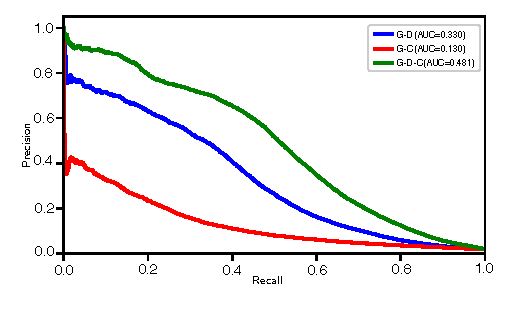
\includegraphics[width=1.0\textwidth]{figure/pr_cureve_u_d_u_c_u_d_c_components.pdf}
	\caption{G-D-C模型、G-C模型和G-D模型P-R曲线对比}
	\label{fig:u_d_c_comparation_pr_curve}
\end{figure}

为了对G-D模型、G-C模型和G-D-C模型进行更为精确的定量评价,本文再次使用二类视网膜糖尿病病变数据集中的$40$张像素级标注图像,进一步证实了以上结论。三者的P-C曲线如图\ref{fig:u_d_c_comparation_pr_curve}所示。可以发现,图中绿色的P-R曲线(G-D-C模型)在紫色(G-D模型)以及红色(G-C模型)P-R曲线上方,在曲线与左侧纵轴和下侧横轴围城的面积方面,绿色曲线显然围住了紫色以及红色P-R曲线,G-D-C模型(绿色曲线)、G-D模型(紫色曲线)和G-C模型(红色曲线)各自P-R曲线对应的AUC分别为$0.330$、$0.130$和$0.481$。这些现象再次表明G-D-C模型在视网膜糖尿病病变图像上的性能表现要优于G-D模型和G-C模型,同时也说明了CNN分类器和判别器的不可或缺行,符合\ref{subsec:model_architecture}小节中对二者的角色设计和期望。

另外,基于\ref{sec:idea_thinking}小节中的朴素思路,我们只使用正常图像训练编码器-解码器,希望编码器-解码器具有重建正常信号的能力,从而间接实现疾病标记物的定位,本文将此素朴思路记为基准方法。然而,在二类视网膜糖尿病病变数据集上得到的AUC为$0.083$,远远低于G-C模型、G-D模型和G-D-C模型在此数据集上得到的结果(三者得到的AUC分别为为$0.130$、$0.330$和$0.481$),三者者均远远高于基准方法,也能说明引入CNN分类器和判别器的必要性,从而再次佐证上述结论。
%(更为直观的实验数据参见表\ref{tab:baseline_compared_diabetic_ds})
%\begin{table}[h]
%	\centering
%	\caption{基准模型、G-C模型、G-D模型和G-D-C模型在二类视网膜糖尿病病变数据集上的实验结果表。表格展示的是通过P-R曲线计算的AUC分数。}		
%	\label{tab:baseline_compared_diabetic_ds}
%	\begin{tabular}{c|c|c|c|c}
%		\toprule[2pt]
%		模型名称 & 基准模型 & G-C模型 &G-D模型&G-D-C模型 \\
%		\midrule[2pt]
%		AUC	& $0.083$&	$0.130$ & $0.330$ & $\textbf{0.481}$	 \\
%		\bottomrule[2pt]
%	\end{tabular}
%\end{table}

\section{对于经过编码器-解码器的视网膜糖尿病病变图像的定量分析}\label{sec:indirect_quantitative_evaluation}
在\ref{sec:bin_dr_ds_experiment}小节和\ref{sec:bin_simulated_ds_experiment}小节中,本文在二类模拟皮肤病病变数据集和二类视网膜病变数据集上利用已有的数据像素级标注进行了定量分析,这方式可看做是一种直接验证的方式。在本节中,本文将从间接角度来再次验证本文提出的模型在处理疾病标记物定位问题的有效性。直观的想法是,在理想情况下,如果一种方法可以准确地定位和去除图像中的生物标记,则去除检测到的生物标记后的图像将不再包含疾病标记物,那么去除检测到的生物标记后的图像将很难与原来的正常图像区分开来。基于以上想法,本文将二类视网膜糖尿病病变数据集按照$80$\%和$20$\%的比例分为训练集和验证集,为下文叙述方便,下文简称该数据集为“原始数据集”,并用训练集数据训练一个ResNet-18二类分类器。随后,对于训练集和验证集,每个图像都被输入到训练之后的编码器-解码器中,所有编码器-解码器的输出图像被收集起来,从而得到一个新的数据集,为了后文叙述方便,本文将该数据集记为“‘正常’数据集”。最后,本文使用原始数据集训练得到的ResNet-18二类分类器对“正常”数据集分类。在此,为了分别衡量编码器-解码器将异常图像输入的转化能力和编码器-解码器对正常图像输入的保持能力,本文使用Recall和Specificity作为分类器的评价标准。相关实验结果如表\ref{tab:quantitative_retinal}所示,前两列表示在原始数据集上的实验结果,后两列表示“正常”数据集上的实验结果。

\begin{table}[h!]
	\begin{center}
		\caption{原始正常数据集和“正常”数据集分类结果} 
		\label{tab:quantitative_retinal}
		\begin{tabular}{c|cc|cc}
			\toprule[2pt]
			& \multicolumn{2}{c|}{原始数据集} & \multicolumn{2}{c}{“正常”数据集} \\
			&  训练集 & 验证集 & 训练集 & 验证集\\
			\midrule[2pt]
			Recall & $0.958$ & $0.936$ & $0.269$ & $0.292$\\ \hline
			Specificity & $0.984$ & $0.964$ & $0.980$ & $0.964$\\
			\bottomrule[2pt]
		\end{tabular} 
	\end{center}
\end{table}

从表\ref{tab:quantitative_retinal}不难看出,对于原始数据集(见表中前两列),ResNet-18分类器不仅在训练集上取得了较高的特异性(Specificity=$0.984$)和召回率(Recall=$0.958$),在测试集上也表现了优异性能(Recall和Specificity分别为$0.936$和$0.964$),说明ResNet-18分类器已经学会了寻找用于分类预测的疾病标记物的特征。另外,表\ref{tab:quantitative_retinal}中后两列显示,大多数“正常”数据集中的异常图像在训练集和验证集上都被错误地归类为正常,导致更低的召回率(训练集和验证集上的Recall分别为$0.269$和$0.292$),说明本文提出的模型能够很好地定位并去除原始异常图像中的疾病标记物,使得ResNet-18二分类器无法将去除疾病标记物的图像与原始正常图像区分开来。另一方面,ResNet-18分类器在正常图像上具有较高的特异性值(训练集和验证集上分别为$0.980$和$0.964$),说明经过编码器-解码器后的正常图像仍然被正确分类为正常图像,这证实了编码器-解码器不会改变正常输入,也从实验角度证明了在\ref{sec:idea_thinking}小节中对编码器-解码器的设想。总之,在原始数据集和“正常”数据集上,无论对于其中的训练集还是验证集,召回率的大幅下降和特异性的小幅下降表明,本文提出的模型可以很好地从图像中去除潜在的疾病标记物,同时保持正常区域不变。从而再次从CNN分类器的角度证明了本文提出的方法的优异性能。
\begin{figure}[h]
	\centering
	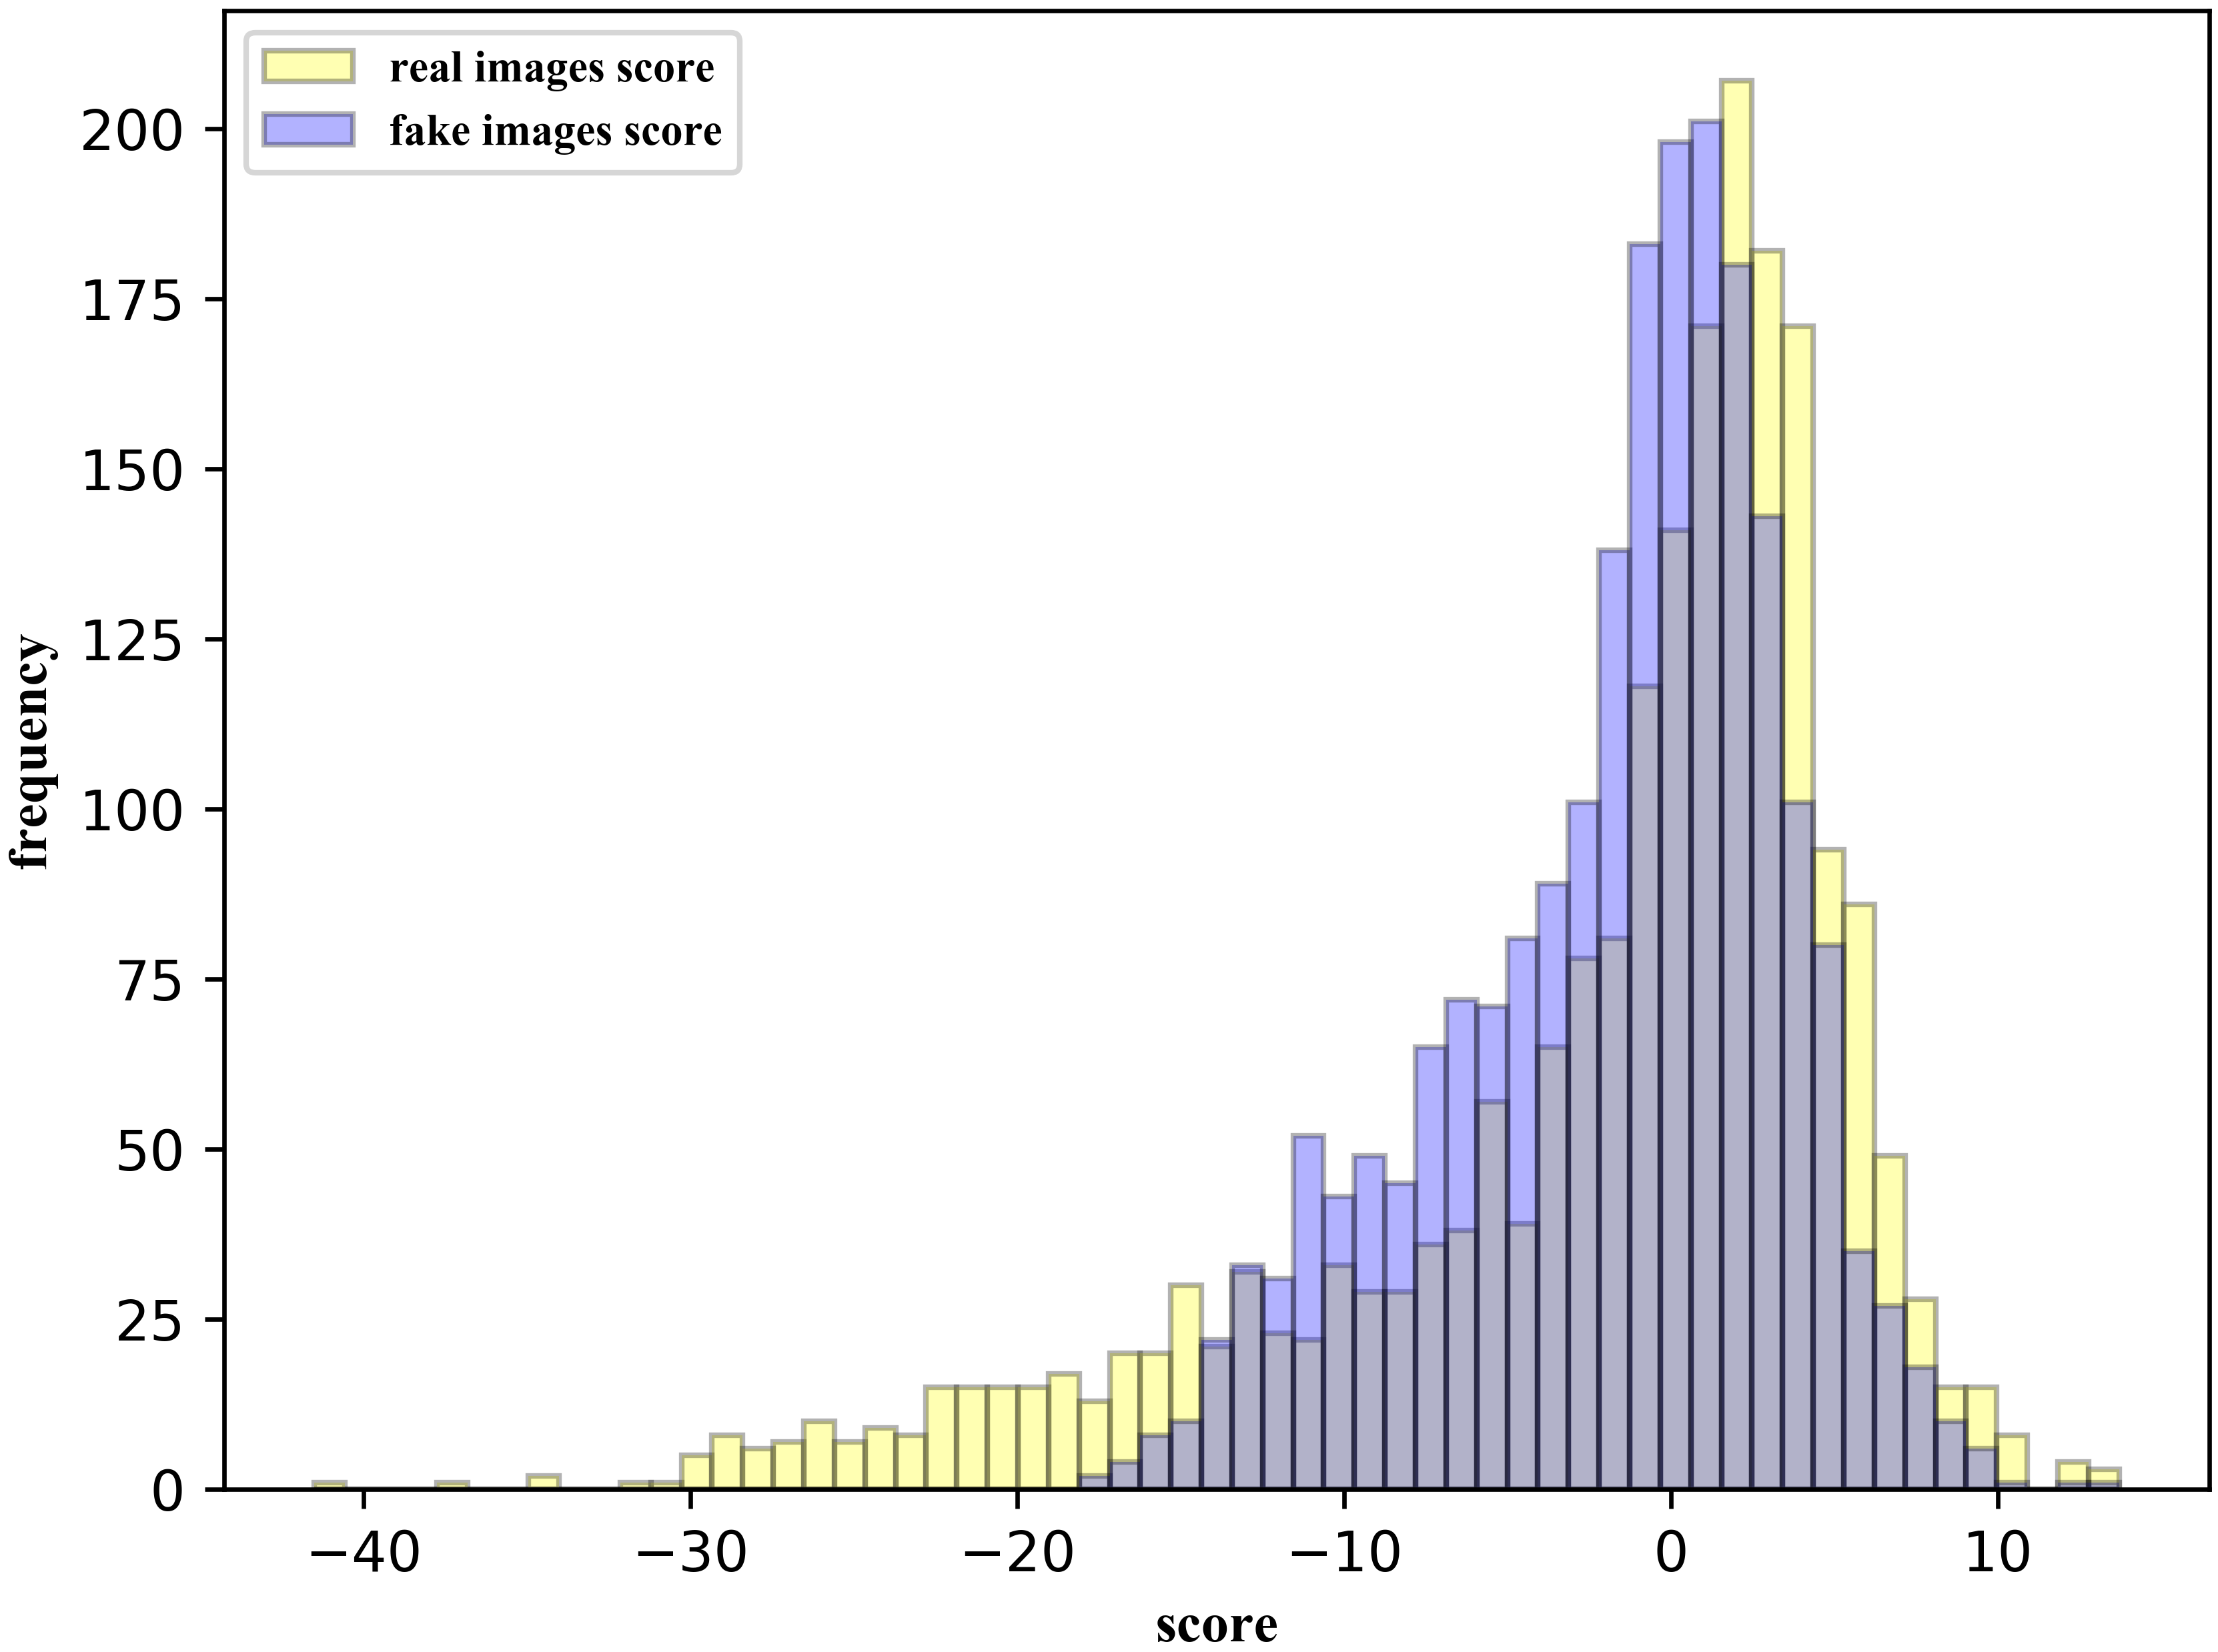
\includegraphics[width=1.0\textwidth]{figure/score_distribution}
	\caption{判别器输出分数频率分布直方图(“正常”数据集作为输入)}
	\label{fig:hist_freq}
\end{figure}
另外,训练结束后,我们还将“正常”数据集中的正常图像和异常图像均送入判别器,判别器输出分数的频率分布直方图如图\ref{fig:hist_freq}所示。图中黄色柱子表示判别器“真”图像输入端的输出分数,蓝色柱子表示判别器“假”图像输入端的输出分数。

不难从直方图中看出,送入判别器的两端分数的频率分布直方图有较大重叠部分,如果暂时不考虑原始图像中的离群点(直方图中靠近下侧横轴最左端的分数),则两者分解输出分数会更加接近。我们还可以根据以上直方图可计算得到,判别器对于“正常”数据集中的正常图像和异常图像输出的平均输出分数分别为$-2.1$和$-1.7$,而在初始参数下,两者的平均分数分别为$-2.2$和$-1.0$,这说明训练结束后,判别器输出端的输入图像相似度得到极大提升(判别器两端输出平均分数的差值大大缩小:$1.2\rightarrow 0.4$)。总之,以上现象可说明,对于正常图像输入,编码器-解码器基本不改变其像素强度;而对于异常图像输入,经过编码器-解码器的输出与不断向正常图像输出靠近,也从判别器的角度间接说明编码器-解码能够比较好地去除原始数据集中的疾病标记物。


\section{对判别器模型结构的探究}\label{sec:dis_arch}
% 原始 D_FPN
% 对比跨层 D_NSC no skiping connection
% 去掉第一个下采样(高分辨率特征 用中间层 不用高分辨率特征融合) D_NLL no feature map from low layer
% 去掉最后一个下采样(不用中间层特征 只用高分辨率)D_NML no feature map from middle layer
在本节内容中,在保持其他设置不变的情况下,本文将设置一系列有关判别器结构的消融实验来探究不同判别结构对于最终定位结果的影响。判别器的网络结构可参见图\ref{fig:discrimintor_architecture},为了后文叙述方便,将原始判别器记作$\mathrm{D}_\mathrm{FPN}(i,j)$。为了探究跨层结构的影响,本文将去掉所有跨层结构的判别器记作$\mathrm{D}_\mathrm{NSC}(i,j)$。在原始判别器中,最后一个全连接层是由第一个下采样单元输出特征、最后一个下采样单元输出特征和最后一个网络单元输出特征融合得到,为了探究来自不同层次和不同分辨率特征融合的影响,本文将去掉第一个下采样单元特征输出而进行特征融合的判别器记作$\mathrm{D}_\mathrm{NLL}(i,j)$,将去掉最后一个下采样单元而进行特征融合的判别器记作$\mathrm{D}_\mathrm{NML}(i,j)$,其中二元组$(i,j)$表示判别器卷积单元总数和其中的下采样单元个数,例如,$\mathrm{D}_\mathrm{FPN}(i,j)$表示一个总共有$7$个网络单元,其中前$4$个网络单元为下采样单元的原始判别器,这也是本文所有实验的默认判别器网络结构设置。关于以上二元组更为直观的含义可参考图\ref{fig:discrimintor_architecture}。另外,本节还探讨了不同深度和下采样单元个数对于原始判别器的影响。接下来,我们在保持其他实验设置不变的情况,按照上述判别器结构依次在二类模拟皮肤病病变数据集上进行测试,最后我们根据实验结果绘制的P-R曲线如图\ref{fig:pr_curve_skin_dis_arch}所示。
\begin{figure}[h]
	\centering
	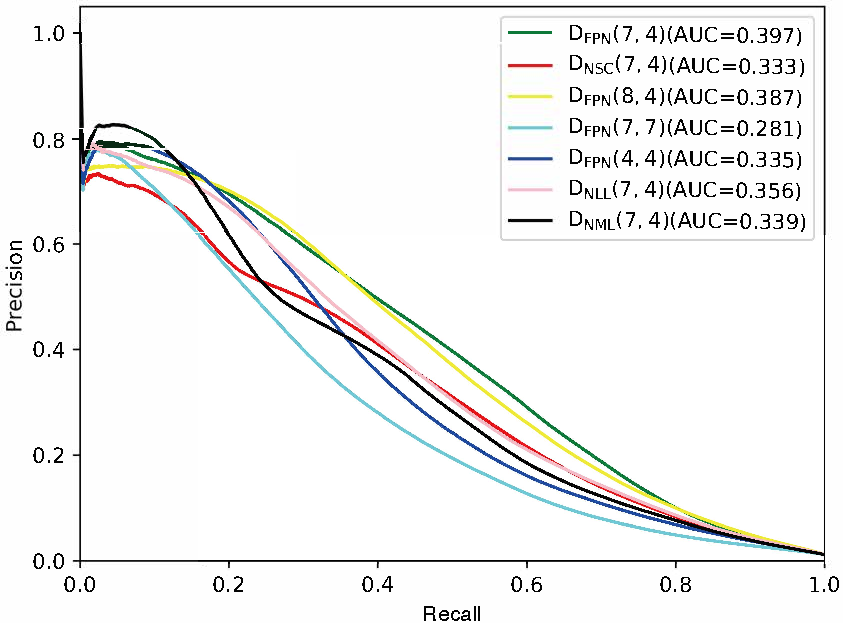
\includegraphics[width=1.0\textwidth]{figure/pr_curve_dis_arch/pr_curve.pdf}
	\caption{不同判别器模型结构P-R曲线对比} 
	\label{fig:pr_curve_skin_dis_arch}
\end{figure}

从上图可以看出,对于默认判别器模型$\mathrm{D}_\mathrm{FPN}(7,4)$(图中绿色曲线),本文提出的模型定位性能最佳,AUC分数最高(AUC=$0.397$)。相比较之下,当去掉默认判别器所有跨层连接时($\mathrm{D}_\mathrm{NSC}(7,4)$,图中红色曲线),性能下降最为严重($0.397\rightarrow 0.333$),这主要是因为网络提取到的浅层高分辨率特征往往对异常图像中尺寸偏小的疾病标记物有着极强语义性。另外,在原始判别器基础上,我们去掉最后一个下采样单元与最后一个全连接层的跨层连接得到$\mathrm{D}_\mathrm{NML}(7,4)$(图中黑色曲线),同理,我们去掉第一个下采样单元与最后一个全连接层的跨层连接得到$\mathrm{D}_\mathrm{NLL}(7,4)$(图中粉色曲线),在以上两种情况下,虽然本文提出的模型的定位性能也有所下降,前者AUC:$0.397\rightarrow 0.339$,后者AUC:$0.397\rightarrow 0.356$,但是AUC分数的下降幅度与$\mathrm{D}_\mathrm{NSC}(7,4)$相比要小($\mathrm{D}_\mathrm{NSC}(7,4)$、$\mathrm{D}_\mathrm{NML}(7,4)$和$\mathrm{D}_\mathrm{NLL}(7,4)$相较于默认判别器模型,AUC分数下降幅度分别为$0.064$,$0.058$和$0.041$),也进一步说明判别器模型的浅层特征对于定位异常图像中分布广泛、大小不一的疾病标记物的重要性,这也是我们在判别器模型中加入跨层结构,让判别器融合不同层次、不同分辨率的特征的主要原因。另外,在默认判别器$\mathrm{D}_\mathrm{FPN}(7,4)$基础上再加入一个卷积单元可得到$\mathrm{D}_\mathrm{FPN}(8,4)$(图中黄色曲线),但就定位性能来看出现了略微下降(AUC分数为$0.387$),这是因为额外引入一个卷积单元虽然没有改变特征图的尺寸,但是对于尺寸较小的疾病标记物就来说,更深的网络意味着更低的语义性,梯度的回传也会变得相对困难。另外,本文针对判别器下采样的次数,本文也设置了相关实验,当判别器模型采用$\mathrm{D}_\mathrm{FPN}(7,7)$(图中青色曲线)时,我们发现本文提出的模型的定位性能最差(AUC=$0.281$)。由于输入图像尺寸为$128\times 128$,实际上判别器的下采样次数最多为$7$次,故随着下采样次数增加,特征图分辨率不断减少,在此过程中,相较于像素数量占绝对优势的正常像素,尺寸较小的疾病标记物的相关信息更难以被提取到,导致本该具备高语义的低分辨率高层特征对于尺寸较小的疾病标记物来说,其语义性大打折扣。反之,当下采样次数过少时,此时的“低分辨率”的高层特征中往往包含很多冗余或者无关干扰信息,故此时的高层特征的语义性也较低,这也是判别器模型采用$\mathrm{D}_\mathrm{FPN}(4,4)$(图中蓝色曲线)时,本文提出的模型的定位性能与默认判别器模型相比也有所下降的原因。而默认判别器模型中由于相比$\mathrm{D}_\mathrm{FPN}(4,4)$又有额外$3$个卷积单元,能过滤与疾病标记物无关的背景信息,增加了“低分辨率”高层特征的语义性,这也是采用默认判别器模型时本文提出的模型的定位性能更优的原因。
%为了更为直观看出以上各个模型之间的定位性能差异,我们将以上判别器模型结构及其AUC分数列在表\ref{tab:dis_arch}中。
%\begin{table}[h]
%	\centering
%	\caption{不同超参数组合下,本文提出的模型在二类视网膜糖尿病病变数据集上计算得到的AUC分数列表。}		
%	\label{tab:dis_arch}
%	\resizebox{1.0\textwidth}{!}{
%		\begin{tabular}{c|c|c|c|c|c|c|c}
%			\toprule[2pt]
%			& $\mathrm{D}_\mathrm{FPN}(7,4)$ & $\mathrm{D}_\mathrm{NSC}(7,4)$&
%			$\mathrm{D}_\mathrm{NLL}(7,4)$&
%			$\mathrm{D}_\mathrm{NML}(7,4)$& $\mathrm{D}_\mathrm{FPN}(8,4)$&
%			$\mathrm{D}_\mathrm{FPN}(7,7)$&
%			$\mathrm{D}_\mathrm{FPN}(4,4)$ \\
%			\midrule[2pt]
%			AUC	& $\textbf{0.397}$ &	$0.333 $ & $0.356$ & $0.339$ & $0.387$& $0.281$ & $0.335$	 \\
%			\bottomrule[2pt]
%		\end{tabular}
%	}
%\end{table}

\section{不同超参数下的实验结果分析}\label{sec:hyper_paras}
为了验证本文提出的模型的超参数鲁棒性(损失函数见等式\ref{equ:model_loss_func}),本文对损失函数中的两个超参数$\lambda_{1}$和$\lambda_{2}$进行测试,旨在找出比较鲁邦的超参数范围。为此,在保证学习率、迭代次数、网络参数初始化等所有相关设置相同的情况下,本文取了$7$种不同的$\lambda_{1}$和$\lambda_{2}$超参数取值,在二类糖尿病病变数据进行了相关测试。这里同样使用P-R曲线及其AUC分数作为评价标准。相关实验结果如图\ref{fig:pr_curve_retinal_hyper_paras}所示。
\begin{figure}[h]
	\centering
	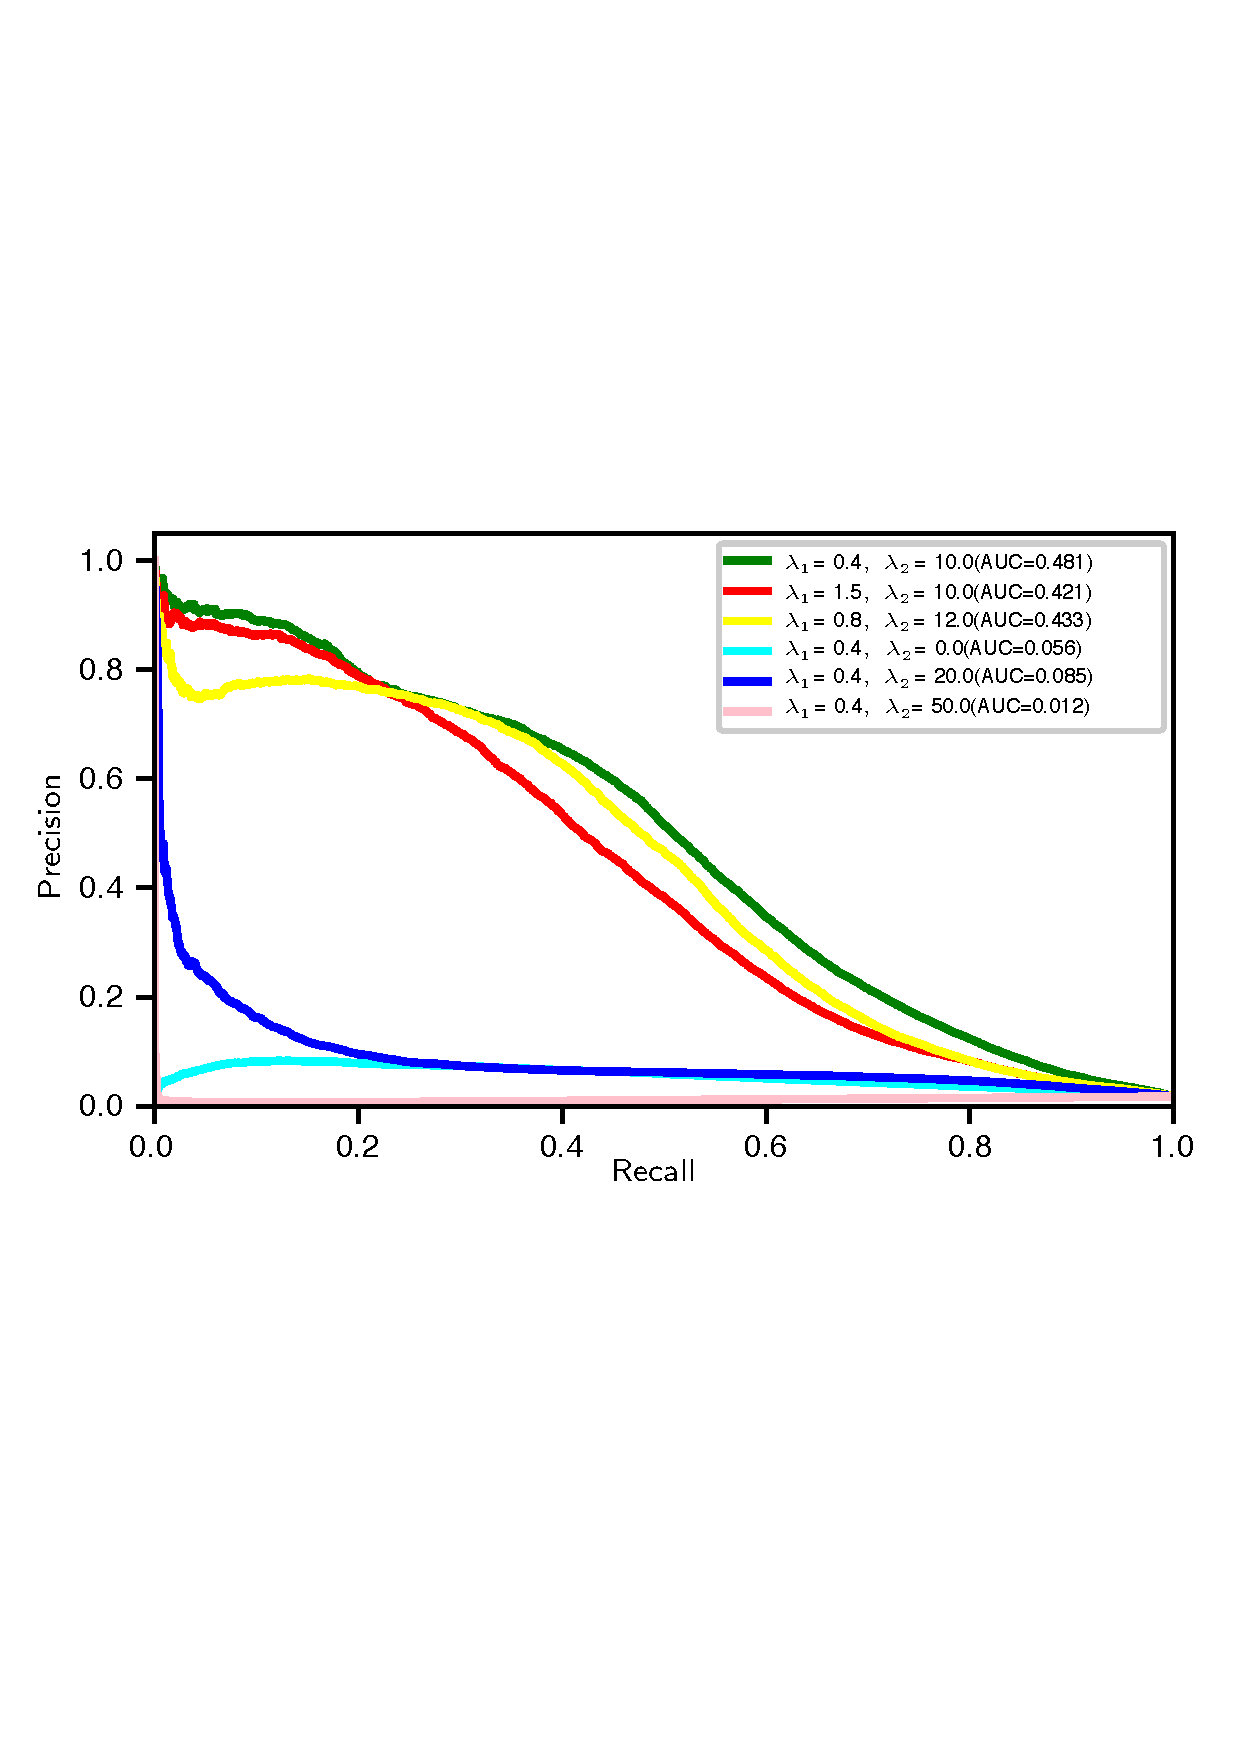
\includegraphics[width=1.0\textwidth]{figure/pr_curve_retinal_hyper_paras/pr_curve.pdf}
	\caption{不同超参数组合下P-R曲线对比} 
	\label{fig:pr_curve_retinal_hyper_paras}
\end{figure}

从图\ref{fig:pr_curve_retinal_hyper_paras}可以看出,在$\lambda_{1}=0.4, \lambda_{2}=10$、$\lambda_{1}=1.5,\lambda_{2}=10$和$\lambda_{1}=0.8,\lambda_{2}=12$这三组超参数设置下,模型性能表现比较稳定,AUC取值分别为$0.481$(图中绿色曲线)、$0.421$(图中红色曲线)和$0.433$(图中黄色曲线)。说明$\lambda_{1}\in [0.4,1.5]$,$\lambda_{2}\in [10,12]$范围内,文本提出的模型的性能比较稳定。另外,注意到$\lambda_{1}=0.4,\lambda_{2}=0$时,本文模型取得较低AUC($0.056$,图中青色曲线),说明损失函数中L1损失对编码器-解码器输入输出约束的必要性(见等式~\ref{equ:model_loss_func})。而当$\lambda_{2}\geq 20$时,本文提出模型的性能也比较差,其中,$\lambda_{2}=20$时,AUC为$0.085$(图中蓝色曲线);$\lambda_{2}=50$时,AUC为$0.012$(图中品红色曲线),这主要是因为当$\lambda_{2}$过大时,在损失函数中真正起主导作用的是L1损失函数,此时,无论对于异常图像还是正常图像输入,编码器-解码器模块的输入输出均变化不大,从而导致疾病标记物定位失败,表现出AUC较低,比较接近基准模型(相关叙述见\ref{sec:g_c_g_d_g_d_c_comparsion}小节)的定位性能。而另一个极端,当$\lambda_{1}\rightarrow 0$时,相当于模型中移去CNN分类器,相关结果在\ref{sec:g_c_g_d_g_d_c_comparsion}小节中已有展示。
%另外,为了更为直观的观察不同超参取值下的模型性能,本文将超参数组合与对应AUC分数列在表\ref{tab:diff_parameters}中。

%\begin{table}[h]
%	\centering
%	\caption{不同超参数组合下,本文提出的模型在二类视网膜糖尿病病变数据集上计算得到的AUC分数列表。}		
%	\label{tab:diff_parameters}
%	\resizebox{1.0\textwidth}{!}{
%		\begin{tabular}{c|c|c|c|c|c|c}
%			\toprule[2pt]
%			& $\lambda_{1}=0.4,\lambda_{2}=10$ & $\lambda_{1}=0.8, \lambda_{2}=10$& $\lambda_{1}=1.5, \lambda_{2}=10$&
%			$\lambda_{1}=0.4,\lambda_{2}=0$& $\lambda_{1}=0.4,\lambda_{2}=20$ & $\lambda_{1}=0.4,\lambda_{2}=50$ \\
%			\midrule[2pt]
%			AUC	& $\textbf{0.481}$ &	$0.421 $ & $0.433$ & $0.056$ & $0.085$& $0.012$	 \\
%			\bottomrule[2pt]
%		\end{tabular}
%	}
%\end{table}
\section{本章小结}
本章主要展示了在二类模拟皮肤病病变数据集和二类视网膜糖尿病病变数据集上的相关实验结果及其分析,与CAM和Grad-CAM,从P-R曲线及其AUC角度看,本文提出的模型可以实现更为精确的疾病标记物定位结果。另外,为了让读者更清楚地理解本文提出的模型的内部情况,本章设计了系列消融实验,例如在\ref{sec:g_c_g_d_g_d_c_comparsion}小节中通过分别去掉CNN分类器和判别器的方式来探究二者在完整模型中所起到的作用。除了直接与CAM和Grad-CAM作比较来证明本文提出的模型的性能优越性,还通过间接方式分别从CNN分类器和判别器进行了进一步验证(参加\ref{sec:indirect_quantitative_evaluation}小节)。最后,还分别设计了两组对比实验分别探究了本文提出的模型的适用超参数范围和判别器结构变化对于整体模型的影响。在两个二类疾病标记物数据集上,相比于CAM和Grad-CAM,本章通过设计了一系列实验证明本文提出的方法在精确定位疾病标记物上的性能优越性。到此,本文提出的模型在二类疾病标记物的精确定位问题叙述完毕。接下来将在第\ref{sec:multi_classes}章中展示本文提出的模型在处理多类疾病标记物的精确定位问题的相关实验结果。如\ref{sec:existing_diffcuities}小节中所描述的那样,由二分类疾病标记物的定位问题到多分类疾病标记物的定位问题并不是一个简单的二类到多类的推广,而是存在诸多难题。在数据集方面,图像数量比较多、图像质量比较高的多类数据集难以收集,而且图像的像素级标注代价高昂的问题依然存在。在模型的训练方面,对于CNN分类器的处理比较容易,将二类交叉熵损失替换成多类交叉熵即可,难点是如何处理判别器,因为对抗生成网络只有正常/异常两个输入端,是否要添加新的判别器来处理新加入的类别,另外,存在多个类别时,如何组织数据训练模型,这些均是值得考虑的问题。接下来,在第\ref{sec:multi_classes}章中,本文将针对以上问题展开相关内容的叙述,同时选取可用于多类疾病标记物精确定位任务相关的数据集,最后展示相关实验结果并对其进行分析。


